\documentclass{beamer}
\usepackage{float}
\usepackage{listings}
\usepackage{subcaption}
\usepackage{amsmath}
\usepackage{hyperref}
\usepackage{rotating}
%ARG Added: Landscape (widescreen) presentation 16:9
\usepackage{beamerthemesplit}
\usepackage[orientation=landscape,size=custom,width=16,height=9,scale=0.5,debug]{beamerposter} 

\hypersetup{colorlinks=true}
\usetheme{rob}
%\usetheme{Boadilla}
%\useinnertheme{circles}
%\useoutertheme{infolines}
%\usecolortheme{whale}


%\title[G4DMC]{Excessive Phonon Energy in G4DMC Events\\[1em]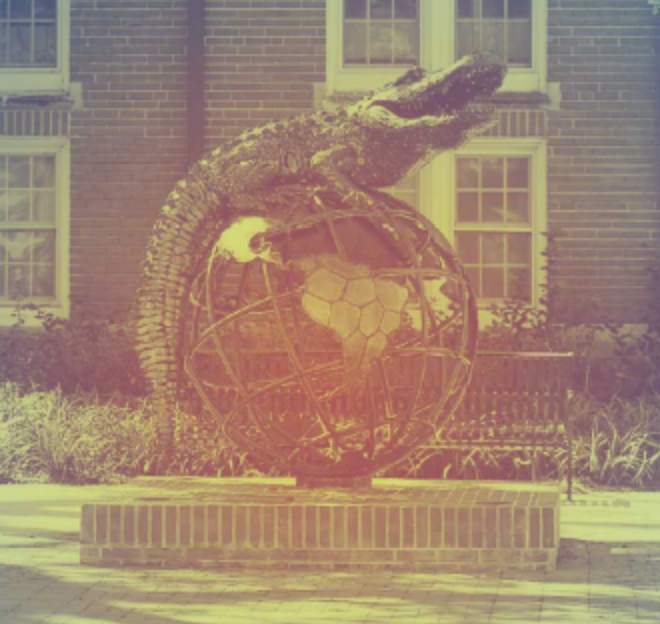
\includegraphics[width=3cm]{gator.png}}

\title[G4DMC]{Excessive Phonon Energy in G4DMC Events}
\titlegraphic{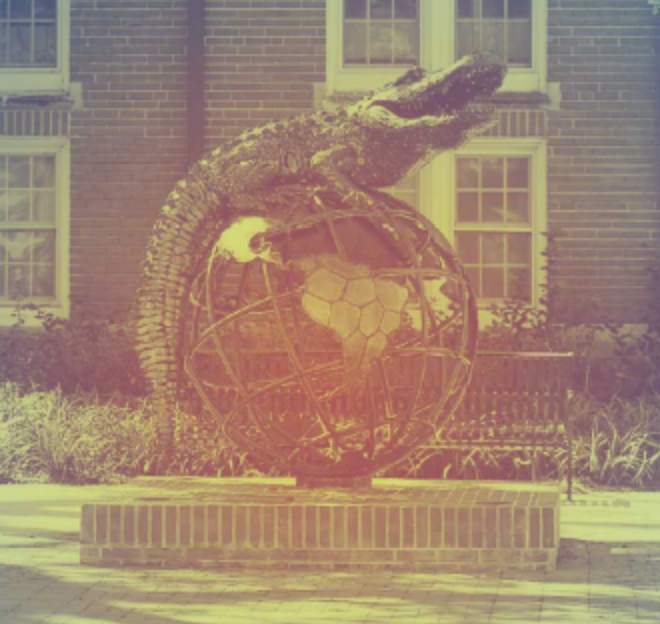
\includegraphics[width=3.5cm]{gator.png}}
%\subtitle{\textbf{Subtitle}}

\author{Rob Agnese}
\institute{University of Florida}
\date{February 27, 2017}



\begin{document}

\begin{frame}[plain, noframenumbering]
    \titlepage{}
\end{frame}

\begin{frame}{The Problem}
    \vfill
    While debugging the track weighting discrepencies, I noticed that
    even without downsampling, we were getting too much energy out from a 
    simulation. \\

    For an electron recoil we should expect:
    \begin{equation}
        E_{phonon} = E_{recoil} + 4 \textrm{volt} \times 
        \textrm{floor}\left(\frac{E_{recoil}}{E_{pair}}\right)
    \end{equation}

    For the 1 keV event I tested, that should be $\sim$ 2.4 keV. G4DMC collected
    a total of $\sim$ 3.1 keV of phonon energy.
    \vfill
\end{frame}

\begin{frame}{Investigation}
    \vfill
    Some immediate consistency checks:
    \begin{itemize}
        \item Charge drift speeds still match data.
        \item Energy partitioner creates correct initial tracks (energies sum to $E_{recoil}$).
        \item Luke phonon emissions conserve energy on case-by-case basis.
    \end{itemize}
    \vfill
\end{frame}

\begin{frame}{Tests}
    \vfill
    We have checked several potential sources of error:
    \begin{itemize}
        \item Use uniform electric field instead of COMSOL field - \textbf{no change}.
        \item Turn off inter-valley scattering (known to be non-physical) - \textbf{no change}.
        \item Create only phonons - \textbf{Correct energy output}!
        \item Shoot exactly one charge carrier pair - \textbf{Excess still present}.
    \end{itemize}
    \vfill
\end{frame}

\begin{frame}{Places Left to Look}
    \vfill
    The bug must be in the charge physics. We've ruled out inter-valley scattering
    and Luke phonon emission. The drift curves also should rule out E-field
    acceleration bugs. There are three processes left:
    \begin{itemize}
        \item DriftBoundaryProcess - When a charge carrier is absorbed, releases
            its kinetic energy as phonons.
        \item DriftRecombinationProcess - When a charge carrier comes to rest
            in the crystal, it is killed and releases half of the gap energy
            as phonons.
        \item EnergyLimiter - When any particle is below its energy threshold,
            it is simply killed and deposits its kinetic energy as NIEL. This
            shouldn't be triggering ever for charge carriers as threshold = 0.
    \end{itemize}
    \vfill
\end{frame}

%ARG Added: Slides 5- 7 
%Credit -- Beamer Presentations: A Tutorial for Beginners (Part 2)—Lists, Columns, Pictures, Descriptions and Tables https://www.overleaf.com/learn/latex/Beamer_Presentations:_A_Tutorial_for_Beginners_(Part_2)%E2%80%94Lists,_Columns,_Pictures,_Descriptions_and_Tables

\begin{frame}
\frametitle{Using Columns}
\begin{columns}
\column{0.5\textwidth}
<text>
\column{0.5\textwidth}
<text>
\end{columns}
\end{frame}


\begin{frame}
\frametitle{Using Columns}
\begin{columns}
\column{0.5\textwidth}
<text>
\column{0.5\textwidth}
\centering 
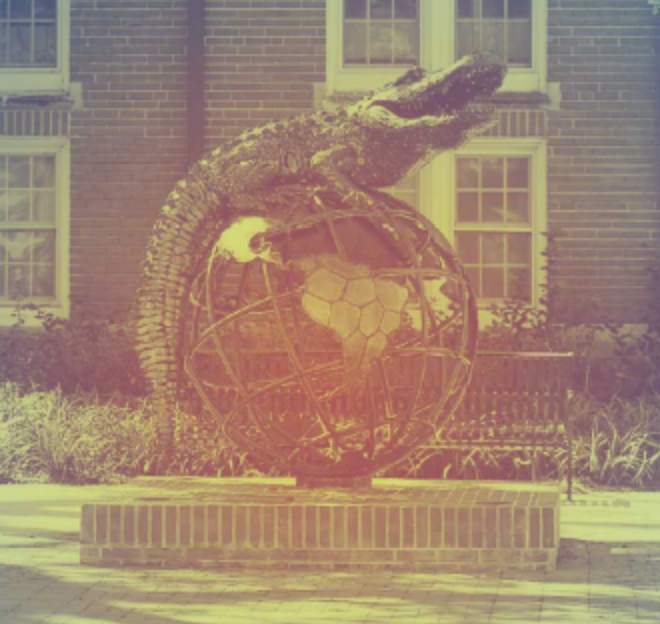
\includegraphics[width=3.5cm]{gator.png}
\end{columns}
\end{frame}



\begin{frame}
\frametitle{Pictures}
\begin{figure}
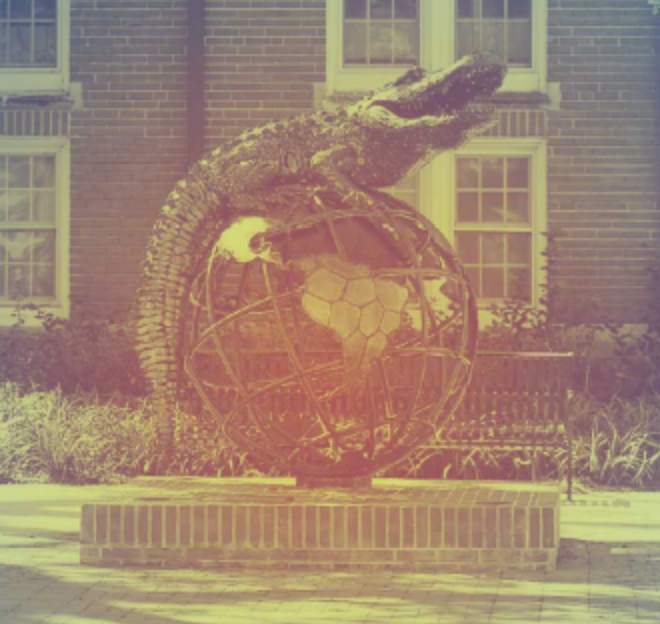
\includegraphics[scale=0.2]{gator.png}
\caption{scaled gator (0.2x)}
\end{figure}
<text>
\end{frame}



\end{document}
